\section[Σταθερή τάση αναφοράς]{Σταθερή τάση αναφοράς $\theta_{ref} = \SI{5}{\volt}$}
\begin{figure}
  \centering
  \begin{subfigure}[t]{\linewidth}
    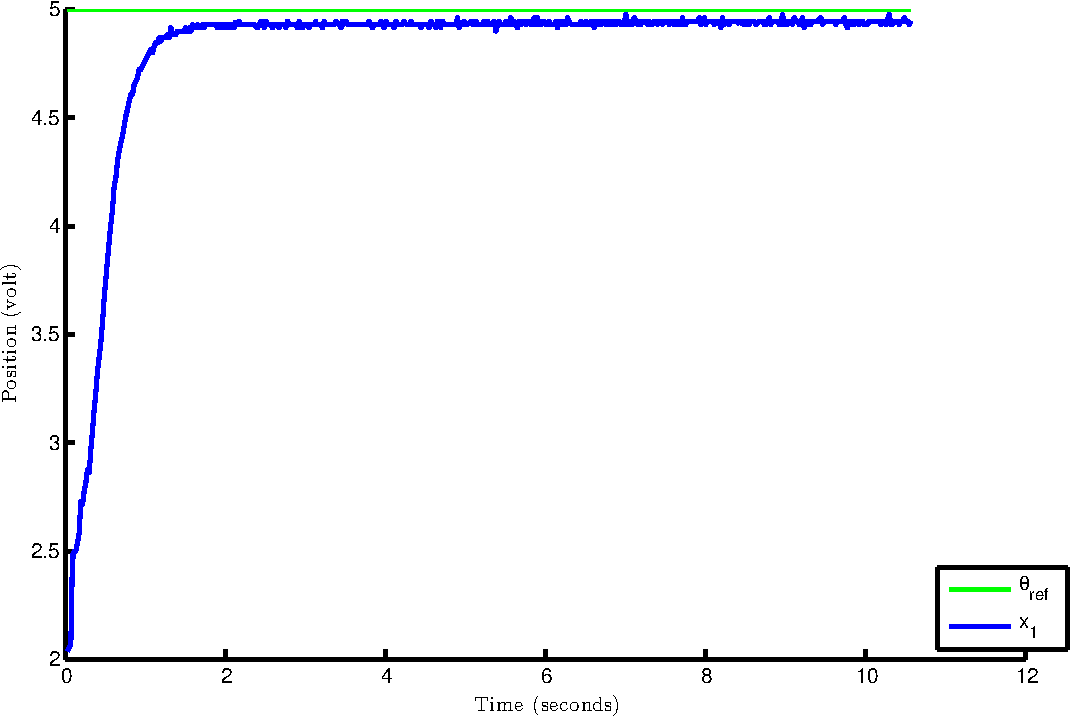
\includegraphics[width=\linewidth, keepaspectratio]{lab2/21-x_1}
    \caption{θέση}
    \label{fig:21-x_1}
  \end{subfigure}\\
  \begin{subfigure}[t]{0.45\linewidth}
    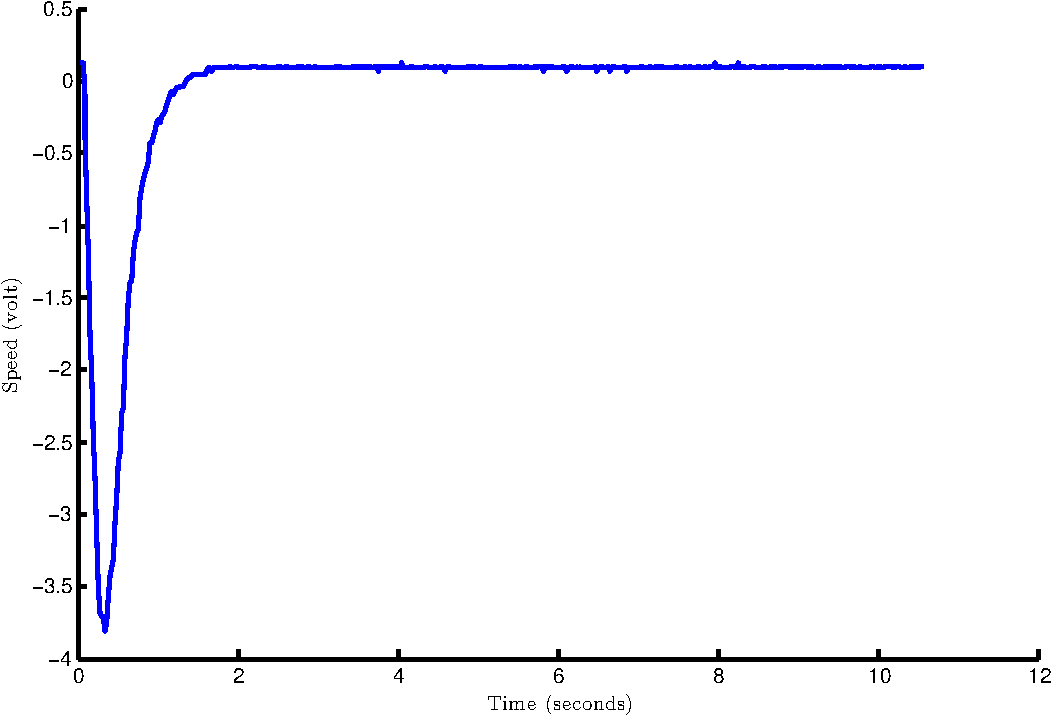
\includegraphics[width=\linewidth, keepaspectratio]{lab2/21-x_2}
    \caption{Ταχύτητα}
    \label{fig:21-x_2}
  \end{subfigure}\hfill
  \begin{subfigure}[t]{0.45\linewidth}
    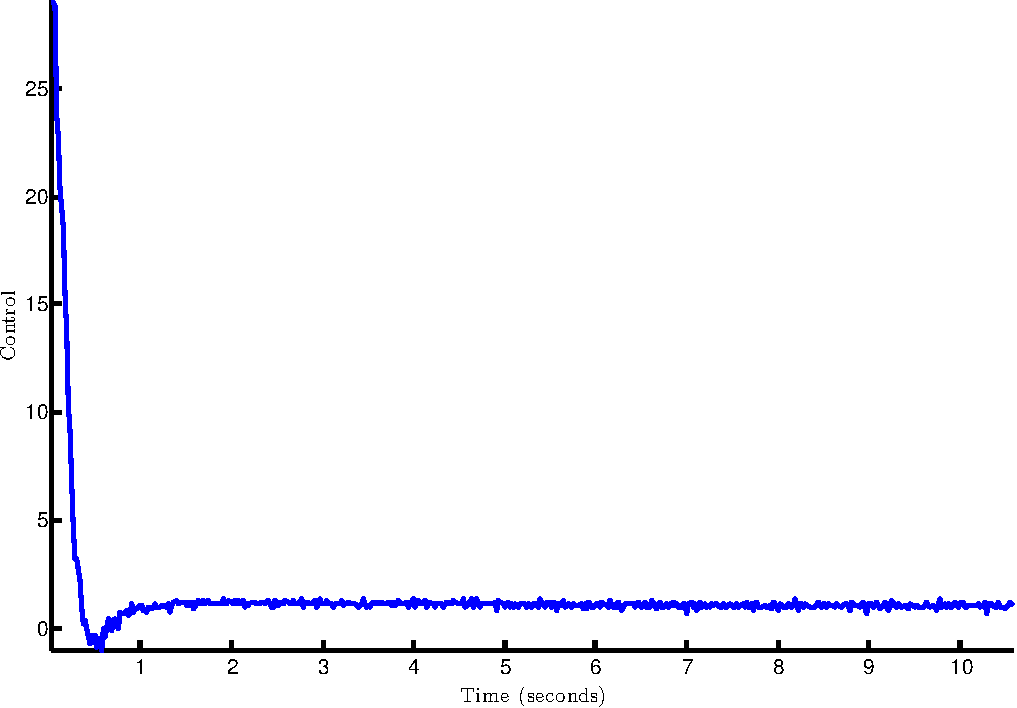
\includegraphics[width=\linewidth, keepaspectratio]{lab2/21-u}
    \caption{Είσοδος ελέγχου}
    \label{fig:21-u}
  \end{subfigure}
  \caption[Γραμμική ανάδραση με σταθερή τάση αναφοράς]{Γραμμική ανάδραση για $\theta_{ref} = \SI{5}{\volt}$}
  \label{fig:21}
\end{figure}
Σύμφωνα με τις παραμέτρους που υπολογίστηκαν παραπάνω γράφτηκε σε κώδικα MATLAB ο ελεγκτής του κινητήρα.
Τα αρχεία που χρησιμοποιήθηκαν είναι τα εξής:
\begin{itemize}
\item \texttt{init\_arduino.m}: Συνάρτηση για την αρχικοποίηση του arduino.
  Παίρνει σαν προαιρετικό όρισμα το \mintinline{MATLAB}!port! αλλιώς χρησιμοποιεί το πρώτο διαθέσιμο.
  Αν δεν υπάρχει διαθέσιμο port χρησιμοποιείται το \mintinline{MATLAB}{port = 'DEMO'} για την εύρεση (συντακτικών)
  σφαλμάτων εκτός εργαστηρίου.

\item \texttt{lab2.m}: Συνάρτηση με τη βασική λούπα και τη λογική ελέγχου.
  Εδώ υπολογίζονται τα κέρδη \mintinline{MATLAB}!k_1!, \mintinline{MATLAB}!k_2!, \mintinline{MATLAB}!k_r!.
  Η επανάληψη δε τερματίζεται όταν η θέση φτάσει τα $\SI{5}{\volt}$ έτσι ώστε να φανεί η ευσταθής συμπεριφορά του συστήματος στη τελική κατάσταση.
  Αντίθετα, ο χρόνος που εκτελείται ο κώδικας εξαρτάται από το χρόνο αποκατάστασης \mintinline{MATLAB}!t_s!.

\item \texttt{lab21.m}: Script για την εύκολη κλήση της παραπάνω συνάρτησης.

\item \texttt{save\_results.m}: Script για την αποθήκευση του workspace της συνάρτησης \mintinline{MATLAB}!lab2!.

\item \texttt{config.m}: Συνάρτηση που επιστρέφει τις παραμέτρους που χρησιμοποιούνται σύμφωνα με τις μετρήσεις του πρώτου εργαστηρίου.

\item \texttt{start\_motor.m} και \texttt{stop\_motor.m}: Απλές συναρτήσεις για την εκκίνηση και το σταμάτημα του κινητήρα.

\item \texttt{adjust\_position.m}: Βοηθητικό script που χρησιμοποιείται για να θέσουμε τον κινητήρα στην αρχική θέση $\theta_0 = \SI{2}{\volt}$ (χειροκίνητα).
\end{itemize}

Η αρχική εκτέλεση του κώδικα δίνει τα διαγράμματα που φαίνονται στην εικόνα~\ref{fig:21}.
Ως τιμές επιλέγονται χρόνος αποκατάστασης $t_s = \SI{1}{\second}$ και $\zeta = 1.1$
όπου $\omega_n = \frac{4}{\zeta t_s}$.
Από τα δεδομένα που προκύπτουν και την εντολή \texttt{stepinfo} του matlab:
\begin{code}
\begin{minted}{text}
    RiseTime: 0.8381
SettlingTime: 10.5757
  SettlingMin: 4.7214
  SettlingMax: 4.9707
    Overshoot: 0
  Undershoot: 0
        Peak: 4.9707
    PeakTime: 7.0047
\end{minted}
\end{code}

\begin{figure}[htb]
  \centering
  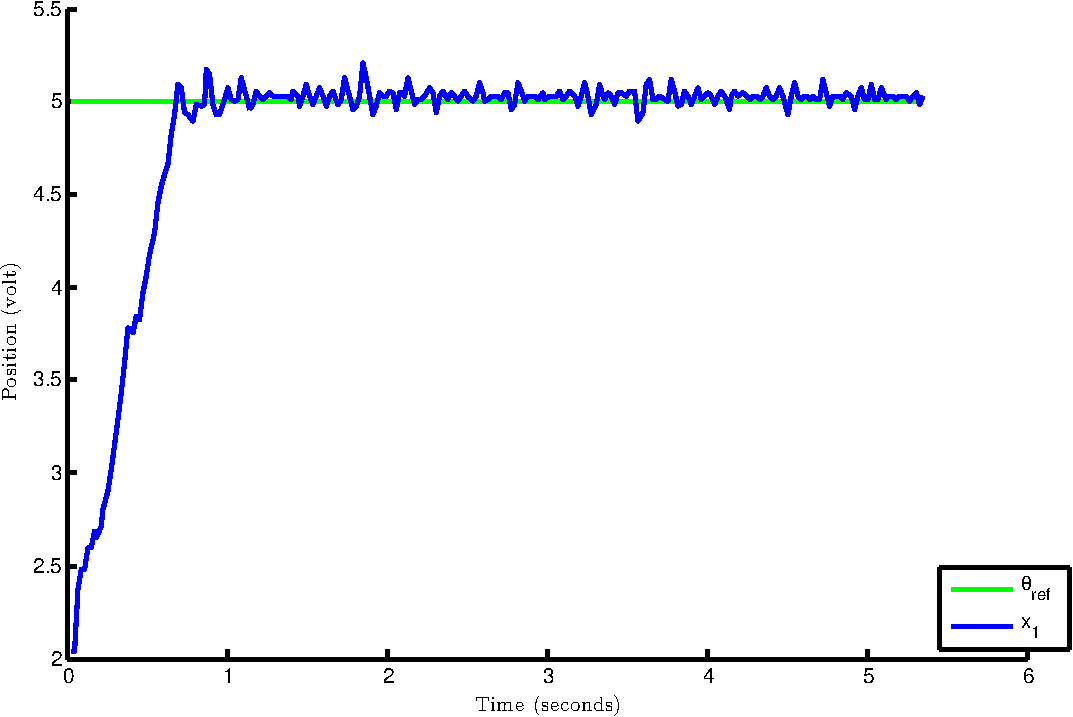
\includegraphics[width=\linewidth]{lab2/21-05-x_1}
  \caption[Γραμμική ανάδραση με μειωμένο χρόνο αποκατάστασης]{Γραμμική ανάδραση για επιλογή $t_s = \SI{0.5}{\second}$}
  \label{fig:21-05}
\end{figure}

Επίσης για $t_s = \SI{0.5}{\second}$ προκύπτουν αποτελέσματα:
\begin{code}
\begin{minted}{text}
    RiseTime: 0.5780
SettlingTime: 5.0980
  SettlingMin: 4.8240
  SettlingMax: 5.2053
    Overshoot: 4.1056
  Undershoot: 0
        Peak: 5.2053
    PeakTime: 1.8518
\end{minted}
\end{code}
και το διάγραμμα θέσης φαίνεται στο σχήμα~\ref{fig:21-05}.

\section{Σφάλμα στη μόνιμη κατάσταση}
\section{Έλεγχος με ύπαρξη μαγνητικού φρένου}
\section[Μεταβαλλόμενη τάση αναφοράς]{Μεταβαλλόμενη τάση αναφοράς $\theta_{ref} = 5 + 2 \sin{\left(\omega t\right)}$}

%%% Local Variables:
%%% mode: latex
%%% TeX-master: "../lab2"
%%% End:
